%% ------------------------------------------------------------------------- %%
\chapter{Test-Driven Development}
\label{cap:tdd}

Métodos ágeis de desenvolvimento de software focam em constante
\textit{feedback}, seja ele da equipe em relação ao cliente, seja da equipe em relação à
qualidade (interna e externa) do código produzido \cite{AgileManifesto}. Por
esse motivo, muitas das práticas sugeridas por métodos ágeis visam aumentar a 
quantidade e a qualidade desse \textit{feedback}; a ideia da programação pareada, por
exemplo, é dar \textit{feedback} sobre o código durante sua escrita.

Test-Driven Development (TDD), popularizada por Kent Beck por meio de seu livro
\textit{TDD: By Example} em 2001 \cite{TDDByExample}, é mais uma das práticas
ágeis na qual o foco é dar \textit{feedback}. TDD tem grande importância durante o ciclo
de desenvolvimento uma vez que, conforme sugerido pelas práticas ágeis, o \textit{design} de um
software deve emergir à medida que o software cresce. E, para responder
rapidamente a essas alterações, é necessário um constante \textit{feedback} sobre a
qualidade interna e externa do código.

TDD é uma prática de desenvolvimento de software que se baseia na repetição de
um pequeno ciclo de atividades. Primeiramente, o desenvolvedor escreve um
teste que falha. Em seguida, deve fazê-lo passar, implementando a
funcionalidade desejada. Por fim, refatora o código para remover toda e qualquer
duplicação de dados ou de código gerada pelo processo.
Simplicidade deve ser também algo intrínseco ao processo; o praticante
deve buscar sempre escrever o teste mais simples que falhe e escrever a implementação mais simples
que faça o teste passar.
Esse ciclo
é também conhecido como 
"Vermelho-Verde-Refatora" (ou \textit{"Red-Green-Refactor"}), uma vez que lembra as cores que um 
desenvolvedor normalmente vê quando faz TDD: o vermelho geralmente significa que
o teste está falhando, e o verde quando o teste foi executado com sucesso.

A prática divide o trabalho do desenvolvedor em duas partes.
A primeira se preocupa em escrever um código que funcione (composta pelas
atividades de escrever o teste e fazê-lo passar). Já a segunda parte se preocupa
com um código claro, expressivo e de fácil manutenção (composta pela atividade
de refatoração). Ron Jeffries fez uma famosa afirmação sobre TDD em que explica
essa divisão: \textit{``Código claro que funciona''} \cite{TDDByExample}. Na
sua opinião, o programador primeiro se preocupa com a parte ``que funciona'', 
para depois deixar o ``código claro''.

As diversas práticas da Programação Extrema provêm \textit{feedbacks} sobre pontos diferentes 
do projeto e em diferentes escalas. 
A velocidade em que a prática de TDD dá \textit{feedback} ao desenvolvedor possibilita que o mesmo
tome decisões sobre o código enquanto o custo de mudança ainda é
baixo. Segundo Vanderburg \cite{vanderburg}, TDD dá \textit{feedback} em questão de
minutos e, em questão de tempo, só é inferior a programação pareada. O gráfico,
baseado no trabalho dele, pode ser visto na Figura
\ref{fig:agile-feedback}.

\begin{figure}
  \centering
  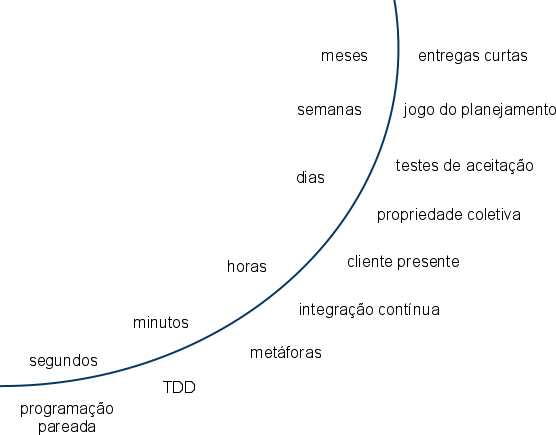
\includegraphics[scale=0.4]{agile-feedback-port}
  \caption{Práticas de XP e Tempo de \textit{Feedback} (baseado em \cite{vanderburg})}
  \label{fig:agile-feedback}
\end{figure}

Este capítulo aborda a prática de TDD, bem como cita
seus efeitos no teste e no \textit{design} do software, conforme relatado pela
literatura.

%% ------------------------------------------------------------------------- %%
\section{Benefícios dos testes}

Uma consequência da prática de TDD é a bateria de testes de unidade gerada.
A prática ajuda o programador a evitar erros de regressão, em que a implementação de
uma nova funcionalidade quebra uma outra funcionalidade já existente no sistema.
Essa bateria também provê segurança durante as
constantes refatorações de código que são feitas durante o processo de
desenvolvimento, e possibilita com que ele altere o \textit{design} e garanta que o
comportamento ainda seja o mesmo. 
A quantidade de código coberto pelos testes também tende a ser alta, uma vez que o
desenvolvedor deve sempre escrever um teste antes de implementar uma nova
funcionalidade. Além disso, por sua execução ser bastante rápida, a bateria é executada
muitas vezes ao dia, dando \textit{feedback} constante ao programador.

Em projetos novos, praticantes de TDD afirmam que sentem menos necessidade da
utilização de recursos de depuração de código \cite{george-williams-experiment} \cite{janzen-arch-improvement}. 
A quantidade de código
escrita entre um teste e outro tende a ser pequena, e caso um teste falhe
inesperadamente, o programador pode simplesmente reverter as alterações para a 
versão anterior estável e começar novamente. Essa abordagem pode muitas vezes
ser mais produtiva do que a atividade de depuração 
\cite{janzen-arch-improvement}. Por essas e outras razões, desenvolvedores afirmam 
que são mais produtivos quando praticam TDD. Apesar de o custo da escrita do teste
existir, a longo prazo o desenvolvedor gasta menos tempo com depurações ou 
erros de regressão, e com isso tem sua produtividade aumentada
\cite{george-e-williams}.

%% ------------------------------------------------------------------------- %%
\section{TDD e \textit{Design}}
\label{cap:tdd-e-design}

É comum relacionar TDD à práticas de testes de software. No entanto, apesar de constar o
termo ``teste'' no nome, TDD não é visto apenas como uma prática de testes.
Embora a criação de testes seja algo intrínseco ao processo, TDD é uma prática
que auxilia o desenvolvedor a criar classes mais flexíveis, mais coesas e
menos acopladas. Os testes são a ferramenta que o programador utiliza para
validar o \textit{design} criado. Por esse motivo, muitos se referem a TDD como
\textit{Test-Driven Design}, ou seja, \textit{design} guiado pelos testes
\cite{tdd-taxonomy}.

Muitos autores como Kent Beck \cite{aim-fire}, Dave Astels \cite{astels-tdd} e
Robert Martin \cite{bob-martin} também afirmam que TDD é na verdade uma prática de
\textit{design} \cite{tdd-taxonomy} \cite{aim-fire}.
Na opinião desses autores, a mudança na ordem do ciclo de
desenvolvimento tradicional, apesar de simples, agrega diversos outros
benefícios ao código produzido: maior simplicidade, menor acoplamento e maior
coesão das classes criadas, levando a um melhor \textit{design}, entre
outros. Ward Cunningham, um dos pioneiros da Programação Extrema, resume essa 
discussão em uma frase: \textit{"Test-First programming is not a testing technique"} 
que, em uma tradução livre, significa \textit{"Escrever primeiro os testes
não é uma prática de testes"}.

%% ------------------------------------------------------------------------- %%
\subsection{Definições incompletas}

Não obstante o foco da prática em \textit{design}, é possível encontrar muitas definições que
não levam isso em conta. Algumas delas consideram apenas a ideia da
inversão da ordem de desenvolvimento, na qual o programador primeiro
escreve o teste e depois escreve o código que o faça passar.

Um exemplo é a definição que pode ser encontrada no livro \textit{JUnit
in Action} \cite{junit-in-action}: \textit{"Test-Driven Development é uma
prática de programação que instrui desenvolvedores a escrever código novo
apenas se um teste automatizado estiver falhando, e a eliminar duplicação. O
objetivo de TDD é 'código claro que funcione'"}.

Embora defina bem o ciclo que a prática impõe ao programador, a definição é incompleta, visto
que ela não captura um dos pontos principais da prática, que é \textit{feedback} no \textit{design}. 
Janzen também levanta esse problema e culpa até o próprio nome da prática, uma vez
que ela possui a palavra ``testes'', mas não contém a palavra \textit{``design''} 
\cite{tdd-really-improve}.

Uma definição mais clara é a de que TDD é a arte de produzir testes
automatizados para código de produção, usando esse processo para guiar o \textit{design} e a programação.
Para cada pequeno pedaço de funcionalidade, o desenvolvedor deve primeiro
escrever um teste que especifique e valide o que o código irá fazer. O
programador então produz somente o código necessário para fazer esse teste
passar. Em seguida, ele refatora (simplifica e clareia) tanto o código de produção
quanto o código de testes \cite{agilealliance-tdd} \cite{tdd-taxonomy}.

%% ------------------------------------------------------------------------- %%
\subsection{Efeitos no \textit{Design} de Classes}

Na abordagem tradicional, programadores escrevem boa parte do código antes de
o testarem. Ao perceberem posteriormente um problema no \textit{design}, o custo para
corrigir pode ser alto demais. Uma vantagem de escrever os testes antes é
possibilitar que o desenvolvedor tome grande parte das decisões de \textit{design}
enquanto o custo de mudança ainda é baixo.

O teste é o primeiro cliente da
classe que o programador ainda está por escrever e isso o faz pensar
melhor a respeito do comportamento que ele espera da classe. Além disso,
programadores contemplam e decidem também sobre a interface (como nomes de
classes e métodos, tipos de retorno e exceções lançadas) que a classe terá
\cite{janzen-saiedian}.
Além disso, ao escrever o teste antes, o programador é encorajado a escrever um
código que seja facilmente testável. Códigos como esse possuem algumas
características interessantes, como a facilidade para invocar o comportamento
esperado, a não necessidade de pré-condições complicadas e a explicitação de
todas as dependências que a classe possui.

Quanto mais difícil for a escrita do teste, maior a chance da existência de
algum problema de \textit{design}. Segundo Michael Feathers, existe uma sinergia muito
grande entre uma classe com alta testabilidade e um bom \textit{design}: se o
programador busca por testabilidade, acaba criando um bom \textit{design}; se 
busca por um bom \texit{design}, acaba escrevendo um \textit{design} mais
testável \cite{feathers-synergy}.

TDD encoraja o programador a escrever componentes fracamente acoplados, de
maneira que eles possam ser testados de maneira isolada e, em um nível maior,
combinados com outros componentes.
Programar voltado para interfaces é uma prática de orientação a objetos há muito
tempo conhecida. Pensar em classes e dar maior foco à maneira com que
elas se relacionam do que com o modo que será implementado determinado
comportamento torna-se mais natural ao praticar TDD \cite{GOOS}. 

%% ------------------------------------------------------------------------- %%
\section{Efeitos na Simplicidade}

TDD sugere que o programador dê sempre pequenos passos (conhecidos pelo termo em
inglês, \textit{baby steps}): deve-se escrever testes sempre para a menor
funcionalidade possível, escrever o código mais simples que faça o teste passar
e fazer sempre apenas uma refatoração por vez \cite{TDDByExample}.

Uma justificativa para tal é a de que, quanto maior o passo que o programador dá, mais
tempo ele leva para concluí-lo e, consequentemente, ele fica mais tempo
sem \textit{feedback} sobre o código. Além disso, faz com que o programador não crie
soluções mais complexas do que elas precisam ser, tornando o código, a longo
prazo, o mais simples possível.

TDD não força o programador a dar "passos de bebê" o tempo todo, mas o
permite dá-los quando achar necessário
\cite{TDDByExample}. Caso o programador esteja confiante sobre o trecho de
código que está escrevendo naquele momento, ele pode dar um passo maior;  porém,
caso ele não esteja tão confiante, a prática o permite ir mais devagar e 
dar "passos de bebê", obtendo \textit{feedback} mais rápido sobre o código que está
escrevendo.

Equipes ágeis optam por não fazer o chamado \textit{big design up-front (BDUF)},
e deixam que o \textit{design} evolua ao longo do tempo, mantendo o código o mais claro e
simples possível, e refatorando sempre que há necessidade. Decisões de
\textit{design} são tomadas com a consciência de que elas serão alteradas no futuro
\cite{is-design-dead}.

Manter o \textit{design} simples não é tarefa fácil, e TDD sugere que o programador
escreva sempre o código mais simples que atenda a necessidade. Somente se a
necessidade crescer, é que o programador deverá evoluir o \textit{design}. Uma decisão de
\textit{design} pode ser mais complicada do que parece e, sem um teste para mostrar isso
rapidamente, o programador dificilmente perceberia o problema \cite{aim-fire}.

Scott Ambler possui uma definição particular sobre como o praticante de TDD lida
com a simplicidade de \textit{design}. De acordo com suas ideias, TDD pode ser definido como
``\textit{TDD = Refatoração + Test-First Design}''. Ainda segundo o referido autor, um programador,
antes de implementar uma nova funcionalidade, deve observar se o \textit{design} atual
possibilita que essa funcionalidade seja implementada de maneira clara. Em caso
afirmativo, o programador segue o ciclo, escrevendo um teste que falha e
fazendo-o passar. Mas, em caso negativo, o programador deve refatorar a parte do
\textit{design} afetado pela nova funcionalidade, de maneira a possibilitar que ela seja
implementada da maneira mais fácil possível \cite{wambler-tdd}. 